%% FEUP THESIS STYLE for LaTeX2e
%% how to use feupteses for MIEIC dissertations
%%
%% FEUP, JCL & JCF,  Wed Oct  4 16:32:24 2017
%%
%% PLEASE send improvements to jlopes at fe.up.pt and to jcf at fe.up.pt
%%

%%========================================
%% Commands: pdflatex pdis
%%           bibtex pdis
%%           makeindex pdis (only if creating an index) 
%%           pdflatex pdis
%% Alternative:
%%          latexmk -pdf pdis.tex
%%========================================

\documentclass[11pt,a4paper,twoside,openright]{report}
\usepackage[utf8]{inputenc}
%\usepackage[latin1]{inputenc}

%%%%%%% English version 

%% MIEIC options
\usepackage[mieic]{feupteses}                  % work version
%\usepackage[mieic,juri]{feupteses}             % juri verrion
%\usepackage[mieic,final]{feupteses}            % final version

%% Additional options for feupteses.sty: 
%% - portugues: titles, etc in portuguese
%% - onpaper: links are not shown (for paper versions)
%% - backrefs: include back references from bibliography to citation place

%%%%%%% Portuguese version

%\usepackage[mieic,portugues]{feupteses}        % work version
%\usepackage[mieic,portugues,juri]{feupteses}   % juri version
%\\usepackage[mieic,portugues,final]{feupteses}  % final version

%% Uncomment the next lines if side by side graphics used
%\usepackage[lofdepth,lotdepth]{subfig}
%\usepackage{graphicx}
%\usepackage{float}

%% Include color package
\usepackage{color}
\definecolor{cloudwhite}{cmyk}{0,0,0,0.025}
%% package to use -> and other symbols
\usepackage{textcomp}

%% Include source-code listings package
\usepackage{listings}
\lstset{ %
 language=C,                        % choose the language of the code
 basicstyle=\footnotesize\ttfamily,
 keywordstyle=\bfseries,
 numbers=left,                      % where to put the line-numbers
 numberstyle=\scriptsize\texttt,    % the size of the fonts that are used for the line-numbers
 stepnumber=1,                      % the step between two line-numbers. If it's 1 each line will be numbered
 numbersep=8pt,                     % how far the line-numbers are from the code
 frame=tb,
 float=htb,
 aboveskip=8mm,
 belowskip=4mm,
 backgroundcolor=\color{cloudwhite},
 showspaces=false,                  % show spaces adding particular underscores
 showstringspaces=false,            % underline spaces within strings
 showtabs=false,                    % show tabs within strings adding particular underscores
 tabsize=2,	                    % sets default tabsize to 2 spaces
 captionpos=b,                      % sets the caption-position to bottom
 breaklines=true,                   % sets automatic line breaking
 breakatwhitespace=false,           % sets if automatic breaks should only happen at whitespace
 escapeinside={\%*}{*)},            % if you want to add a comment within your code
 morekeywords={*,var,template,new}  % if you want to add more keywords to the set
}

%MJPC TabelasPlease add the following required packages to your document preamble:
 \usepackage[normalem]{ulem}
 \useunder{\uline}{\ul}{}

%% Uncomment to create an index (at the end of the document)
%\makeindex

%% Path to the figures directory
%% TIP: use folder ``figures'' to keep all your figures
\graphicspath{{figures/}}

%%----------------------------------------
%% TIP: if you want to define more macros, use an external file to keep them
%some macro definitions

% format
\newcommand{\class}[1]{{\normalfont\slshape #1\/}}

% entities
\newcommand{\Feup}{Faculdade de Engenharia da Universidade do Porto \,}
\newcommand{\Ess}{Escola Superior de Saúde \,}
\newcommand{\doc}{disorders of consciousness \,}
\newcommand{\Mcs}{Minimally Conscious State \,}
\newcommand{\espaco}{\vspace{1.8mm}}
\newcommand{\para}{}
\newcommand{\svg}{\class{SVG}}
\newcommand{\scada}{\class{SCADA}}
\newcommand{\scadadms}{\class{SCADA/DMS}}

%%----------------------------------------

%%========================================
%% Start of document
%%========================================
\begin{document}

%%----------------------------------------
%% Information about the work
%%----------------------------------------
\title{Title of the Dissertation}
\author{Name of the Author}

%% Uncomment next line for date of submission
%\pdisdate{July 31, 2008}

%%Uncomment next line for copyright text if used
%\copyrightnotice{Name of the Author, 2008}

\supervisor{Supervisor}{Name of the Supervisor}

%% Uncomment next line if necessary
%\supervisor{Second Supervisor}{Name of the Supervisor}

%% Uncomment committee stuff in the final version 
%\committeetext{Approved in oral examination by the committee:}
%\committeemember{Chair}{Doctor Name of the President}
%\committeemember{External Examiner}{Doctor Name of the Examiner}
%\committeemember{Supervisor}{Doctor Name of the Supervisor}

%\committeetext{Aprovado em provas públicas pelo Júri:}
%\committeemember{Presidente}{Nome do presidente do júri}
%\committeemember{Arguente}{Nome do arguente do júri}
%\committeemember{Vogal}{Nome do vogal do júri}

%% Uncomment signature line in the final on paper version
%\signature

%% Specify cover logo (in folder ``figures'')
\logo{uporto-feup.pdf}

%% Uncomment next line for additional text below the author's name (front page)
\additionalfronttext{Preparação da Dissertação}

%%----------------------------------------
%% Preliminary materials
%%----------------------------------------

% remove unnecssary \include{} commands
\begin{Prolog}
  \setlength{\parindent}{4em}
\chapter*{Abstract}


\hspace{4em} People with disorders of consciousness (DOC) are vulnerable to misdiagnosis which can negatively affect their rehabilitation process. The incorrect diagnosis of people with DOC is common, reaching 43 \%. This has possible implications for decisions regarding the provision of health care to this group. Diagnosis of this population depends on the assessment of their behavioral responses to stimuli. The intentionality and types of behavior exhibited by people in a vegetative state (VS) and a minimally conscious state (MCS) can be difficult to distinguish and subtle signs of consciousness can go unnoticed.
It is widely recognized that the use of standardized and sensitive behavioral assessment scales, such as the Sensory Modality Assessment and Rehabilitation Technique (SMART), can help healthcare professionals to identify subtle signs of awareness.
SMART is an assessment tool that combines communication, motor and sensory modalities to diagnose the condition of patients who have suffered severe brain injuries. This method is quite credible and accepted by the healthcare community that deals with this clinical population. It requires and consumes many resources in making the diagnosis.

However, less experienced SMART assessors can be misled by some types of patient responses and even in the analysis of session data, namely in different diagnostic limit zones. Hence a second opinion based on Machine Learning can prove to be very useful. In addition, diagnosis is made session by session and the cumulative diagnostic certainty as the sessions progress.
This tool can be detected as well as the expert assessors, in the future it can be very useful to detect in advance (in a smaller number of sessions) the state of consciousness of the patient to be analyzed.

SMART evaluation has already been explored with statistical software such as statistical package for the social sciences (SPSS) combining analysis methods and techniques such as analysis of variance (ANOVA), etc.
So far, no machine learning methods have been found in partnership with this technique and diagnostic tools (SMART).  

The best diagnosis, through a second opinion performed by the machine, is expected to increase the confidence level in decision-making by SMART assessors. More protected and less subject to criticism of negligence, data that possible errors if detected, can be bridged and safeguarded or at least become noticeable therefore, it leads to higher hit rates. Minimizing the allocation of time to human resources for this specific task, can be beneficial for these professionals due to the useful / effective time to perform tasks (elimination of extra hours to do a task that was previously done).
Institutions: speeds up the prognosis and diagnosis process, making it financially convenient to make professionals more available, resulting in greater performance and efficiency, with the possibility of performing other essential tasks.\\


\vspace*{10mm}\noindent
\textbf{Keywords}: Machine Learning, disorders of consciousness, diagnosis, SMART, minimally conscious state, vegetative state, brain injury,

\chapter*{Resumo}
\hspace{4em} Pessoas com perturbações de consciência (PdC) são vulneráveis a diagnósticos errados que podem afetar negativamente o seu processo de reabilitação. O diagnóstico incorreto de pessoas com PdC é comum, podendo atingir os 43\%. Isto acarreta possíveis implicações nas decisões relacionadas com a prestação de cuidados de saúde desta população. o diagnóstico desta população depende da avaliação das suas respostas comportamentais a estimulação. A intencionalidade e os tipos de comportamentos exibidos por pessoas em estado vegetativo e estado de consciência mínima, podem ser difíceis de distinguir e sinais subtis de consciência podem passar despercebidos. É amplamente reconhecido que o uso de escalas de avaliação comportamental padronizadas e sensíveis, tal como o Sensory Modality Assessment and Rehabilitation Technique (SMART), pode ajudar os profissionais de saúde a identificar sinais subtis de consciência. 
O SMART é um instrumento de avaliação que combina funções comunicacionais, motoras e de aferição de sentidos para diagnosticar o estado de pacientes que sofreram lesões cerebrais graves. Este método é bastante credível e aceite pela comunidade da área da saúde  que lida com esta população clínica. Ele requer e consome muitos recursos na elaboração do diagnóstico.

Contudo, avaliadores SMART menos experientes podem ser induzidos em erro por algum tipos de respostas dos pacientes e mesmo na análise dos dados das sessões nomeadamente em zonas limite de diagnósticos distintos. 
Daí uma segunda opinião com base em Machine Learning pode vir a ser muito útil. Além disso, o diagnóstico é feito sessão a sessão sendo a certeza de diagnóstico cumulativa no progredir das sessões.

Esta ferramenta se detetar tão bem como os avaliadores expert, pode no futuro ser muito útil a detetar antecipadamente (num menor número de sessões) o estado de consciência do paciente analisado.
- A avaliação SMART já foi explorada através de software estatístico como SPSS usando métodos e técnicas de análise ANOVA, etc.
Até ao momento  não foram encontrados  métodos de machine learning em parceria desta técnica e ferramenta de diagnóstico (SMART).  
 
  Melhor diagnóstico, através de uma segunda opinião realizada pela máquina é expectável que aumente o índice de confiança na sua tomada de decisão por parte dos avaliadores SMART . Mais resguardados e menos sujeitos a críticas de negligência, dados que possíveis erros se detectados, possam ser colmatados e salvaguardados ou pelos menos se tornem perceptíveis portanto, conduz a taxas de acerto mais elevadas. Redução dos tempos de alocação a recursos humanos destinados a esta tarefa específica, pode ser benéfico para estes profissionais pelo tempo útil de realização de tarefas (eliminação das horas a mais a fazer uma tarefa já realizada outrora). 
Instituições: agiliza o processo de prognóstico e diagnóstico, financeiramente conveniente tornar profissionais mais libertos consequente maior rendimento e eficácia com possibilidade de realização de outras tarefas primordiais.

\vspace*{10mm}\noindent
\textbf{Keywords}: Aprendizado Máquina, Perturbações de consciência PdC,diagnóstico de consciência, SMART, estado de consciência mínimo, estado vegetativo, lesão cerebral
  % the abstract
  \chapter*{Acknowledgements}
%\chapter*{Agradecimentos}

Hello world!

I want to thank FEUP for the fantastic conditions of labour, the people who work here and people (students like me) by promoting activities that enable the development of areas of our interest.
Dedicated to the people who wants to learn and people with a desire to teach in general. It moves the world.

Above all, I would like to thank the fantastic synergies of the Group Coordinator (VCMI) and supervisor Prof. Jaime Cardoso  as well the Institutional Coordinator of the Superior School of Health of Porto in name of Prof. Nuno Rocha and Prof. Liliana Teixeira of Polytechnic of Leria as the promoters of this interesting idea. 

I want to thank humanity or friendship, the exchange and debate of ideas that exist in the world, which somehow inspires us, gives us encouragement in the most difficult moments and decisions and, on the other hand, gives greater meaning to life, shares happiness and other important feelings with us and vice versa. The power that positive influence can have in one another's lives.
The intrinsic willpower that makes us think, research, understand, solve problems and also make us ask for help and listen.
My thanks to family, affective, academic/professional, community, financial, sports and health support in general, without you it was not the same thing.

\vspace{10mm}
\flushleft{Manuel Curral}
   % the acknowledgments
  \cleardoublepage
\thispagestyle{plain}

\vspace*{5cm}

\begin{flushright}
  \textsl{``You can't stop the waves, but you can learn to surf.
  ''}\\
\vspace*{1.5cm}
    Jon Kabat-Zinn
    
\vspace*{3.5cm}    
    \textsl{``O Universo criou um cérebro para permitir ver-se a si mesmo, para estar consciente de si mesmo.
  ''}\\
  \vspace*{1.5cm}
  Henry Markram
    
\end{flushright}
     % initial quotation if desired
  \cleardoublepage
  \pdfbookmark[0]{Table of Contents}{contents}
  \tableofcontents
  \cleardoublepage
  \pdfbookmark[0]{List of Figures}{figures}
  \listoffigures
  \cleardoublepage
  \pdfbookmark[0]{List of Tables}{tables}
  \listoftables
  \chapter*{Abbreviations}
\chaptermark{ABBREVIATIONS}
%\chapter*{Acrónimos}
%\chaptermark{ACRONIMOS}


\begin{flushleft}
\begin{tabular}{l p{0.8\linewidth}}

\iffalse
API      & Application Programming Interface\\
\fi
ANOVA    & Analysis of Variance \\
DOC      & Disorders of Consciousness\\
DRS      & Disability Rating Scale\\
GCS      & Glasgow Coma Scale\\
ICC      & Intra Class Correlation\\
fMRI     & functional Magnetic Resonance Imaging\\
MCS-     & Minimally Conscious State Minus\\
MCS+     & Minimally Conscious State Plus\\
MMN      & Multifocal Motor Neuropathy \\
NN       & Neural Network \\
SMART    & Sensory Modality Assessment and
Rehabilitation Technique\\
WNSSP    & Western Neuro Sensory Stimulation Profile\\
TBI      & Traumatic brain injury\\
VS       & Vegetative State\\

WWW      & \emph{World Wide Web}
\end{tabular}
\end{flushleft}

  % the list of abbreviations used
\end{Prolog}

%%----------------------------------------
%% Body
%%----------------------------------------
\StartBody

%% TIP: use a separate file for each chapter
\chapter{Introduction} \label{chap:intro}

\section*{Context} \label{sec:context} 
% with * not numerate the title

Consciousness is the individual's ability to be aware of the knowledge of self and the environment. Furthermore, the ability to respond to various voluntary internal and
external stimuli \citet{https://doi.org/10.1196/annals.1440.013}.
In basic neurological terms, it is composed of awareness and wakefulness \citet{zheng2017disentangling}.
The different states of consciousness are represented in the table
\ref{tab:my-table}.

\begin{table}[!htb].
\begin{tabular}{lccll}
\cline{3-3}
\multicolumn{1}{c}{{Condition}}             & \multicolumn{1}{l|}{\textbf{Wakefulness}} & \multicolumn{1}{l|}{\textbf{Awareness}} &  &  \\ \cline{3-3}
Coma                                            & -                                         & -                                       &  &  \\ \cline{1-3}
\multicolumn{1}{|l|}{Vegetative State}          & \multicolumn{1}{c|}{+ to ++}              & \multicolumn{1}{c|}{-}                  &  &  \\ \cline{1-3}
\multicolumn{1}{|l|}{Minimally Conscious State} & \multicolumn{1}{c|}{+ to ++}              & \multicolumn{1}{c|}{+}                  &  &  \\ \cline{1-3}
Emerged from Minimally Conscious State          & ++                                        & ++                                      &  & 
\end{tabular}
\caption{Disorders of consciousness categorization}
\label{tab:my-table}
\end{table}
\vspace{0.2cm}
Brain Injury (BI)  is head injury that damage in the brain and his complex connections. 

This causes
problems with how a person can
think and interact with the world around
him or her. Following a brain injury, there are
specific cognitive skills that are no
longer functioning in the same capacity.
Perception, observation and
recognition of information are deeply affected.

There are events that damage areas of the brain that control parts of the human body. And the patient's faculties are conditioned.
The origin of brain injuries can be: 
\begin{itemize}
    \item acute: as in a virus or hemorrhage  \item traumatic: like road accidents, impacts where there are head injuries  \item non-traumatic: such as drowning, sudden attacks on organs and consumption of substances harmful to the body
\end{itemize} 
That cause brain damage that leads to consequences in terms of disturbing the person's consciousness\cite{teixeira2020disorders}.

After coma, the rates of diagnostic errors, namely in the distinction between vegetative state (VS) and the minimally conscious state (MCS), are high  $\approx 40$ \cite{andrews1996misdiagnosis}  \cite{ gill2004sensory} \cite{schnakers2009diagnostic}. 

The diagnosis of the condition of the patient who suffers brain damage is made using scales to assess the behavioural response to stimulation:
CRS-r, SMART, WHIM, WNSSP, Rancho levels physicians etc. \label{behscales}
With technological advancement and the spread of its use, neuronal imaging technologies such as:
   functional magnetic resonance imaging (fMRI),
   electroencephalogram (EEG)
   positron emission tomography (PET).

  It has been possible to leverage the discovery and knowledge in the area of neuroscience and the identification, consequent diagnosis of the cerebral behavior of patients. This helps a lot in studying %\doc
  DOC because it demonstrates the level of responsiveness that could not be obtained by the behavior scales already mentioned. \ref{behscales}
  
  VS is defined as the absence of self-awareness and the environment. Behaviours are limited to reflexive activities indicating no purposeful movement, neither experience of suffering or evidence of comprehension \citet{multi1994medical}
  
  %\Mcs
  MCS is serious but does not represent a complete lack of awareness resulting  from widespread damage to the telencephalon (the part of the brain that controls thinking and behavior).
  The intentionally and types of behavior exhibited by people in a VS and a MCS,
 can be challenging to distinguish, and subtle signs of consciousness can go unnoticed.
It is widely recognized that the use of standardized and sensitive behavioral assessment scales
such as the Sensory Modality Assessment and Rehabilitation Technique (SMART), can
help healthcare professionals identify subtle signs of awareness.



\section{SMART} \label{sec:smart}

SMART is an assessment tool that combines communication, motor and sensory modalities to diagnose patients who have suffered severe brain injuries \citep{DaConceicaoTeixeira2018}.

Five levels: no response, reflex response, withdrawal response, localized response and differentiated response

Advantage:

This method is entirely credible and accepted by the healthcare community that deals with this clinical population.


Disadvantage:


It requires and consumes many resources in making the diagnosis.

\section{Diagnostic tools} \label{Diagnostic}

Neuroscientific technologies, experimental methods study the patients' brain processes through many devices, in specific: 

Neuroimaging, psychophysical techniques or psychological tests are used to study processes such as learning, attention, memory, or emotion \cite{Corchs2019}.
\espaco

The following stand out:

 
\begin{itemize}


\item Electroencephalogram (EEG)

Electroencephalography is a simple, non-invasive technique based on the recording and evaluating brain activity using electrodes placed on the skull surface. The (EEG) is the record that results from the measurement of the electrical potentials of the brain. EEG shows the electrical fluctuation in the different locations of the cortex \cite{Bender2015}. However it has the disadvantage of having an insufficient resolution to register the neuronal activity in deeper brain structures, such as the \textit{nucleus accumbens} related to the processing of emotions\cite{Lang2010}. %\citep{8701676}. 

Study using MMN tomography technique resulting in classification of patients with DOC in figure \ref{ferramentaMMN}
\begin{figure}[h!]
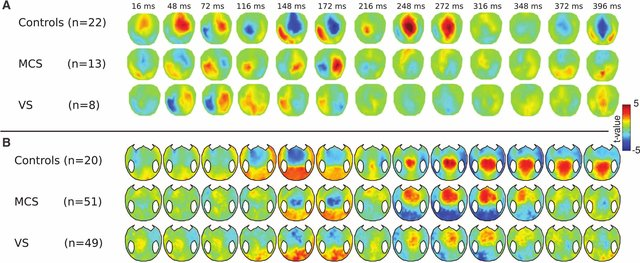
\includegraphics[scale=0.7]{figures/MMN-topography-in-patients-with-disorders-of-consciousness-and-in-healthy-controls-The_W640.jpg}
\caption[MMN topography in patients with disorders of consciousness and in healthy controls. The figure shows a comparison of (A) t test maps from Boly et al. (1) for the MMN (comparison of deviant and standard trials) with (B) similar maps obtained from 120 recordings collected in the past three years in Lionel Naccache's laboratory, Hôpital de la Salpêtrière, Paris]{MMN topography in patients with disorders of consciousness and in healthy controls \cite{King2011}
\cite{Boly2011}} %legenda imagem no indice e no texto
\label{ferramentaMMN}
\end{figure}

\item  (Functional) Magnetic Resonance

 It is a method of diagnosis and fundamental research in Market research Analyzing emotions Planning surgery Brain mapping neurosciences.\citep{fmri} It allows the analysis of the subjects' response to different activities or stimuli. Magnetic resonance imaging is a non-invasive technique used to obtain information about the subjects' response to different stimuli (very common in research and analysis of neurological diseases such as Alzheimer's Disease and also for soft tissue injuries and inflammation). This technique evaluates the activation and the emotional state of the subject when exposed to certain stimuli. \cite{noauthor_fmri_nodate}
 
 
\item  GSR (galvanic skin response)

Measurement of the galvanic response is done by placing
electrodes on the fingers. Studies measure resistance
skin and its conductance.

A GSR amplifier applies constant tension to the skin,
of such a low voltage that the individual cannot
perceive it through electrodes. The current generated in the
skin by tension can be detected and recorded. The output of the GSR amplifier determines the conductance.
The conductance of the skin gives feedback on the body's response to the stimulus, it is widely used in post-coma and coma phases
\cite{Altntop2021,Luaute2018}.



\item  Eye-tracking

 Eye-tracking refers to recording the movements of an individual's eye while examining a visual stimulus. In broad, it is responsible for measuring eye movements using a camera that quantifies them. Modern eye trackers record eye position and movement using contrast to locate the central point of the pupil and create a reflection of the cornea using infrared light. It is possible to perform the analysis of the position of the gaze and the movement of the eyes in three-dimensional environments.
Eye-tracking techniques apply to domains where interaction and interests matter,
looking to sell or immerse to improve the customer or user experience. In medicine, it is essential to recognize behaviours and patterns to investigate further and be able to characterize\cite{Ting2014}.


\item  Face reading

 Facial expressions are one of the most robust  visual methods for conveying emotions. The face plays a crucial role in the cognitive processes of individuals since the signs that show facial expressions denote internal states or emotions. The analysis of facial expressions provides valuable information when combined with other tools that allow sensory information collection, such as eye-tracking or EEG .

\end{itemize}


\espaco




Research continues on clinical tools such as (fMRI) with improved diagnostic certainty and prognostic applications. There are 3 main factors that influence the prognosis of patients in the Vegetative State (VS) and the patient's minimum state of consciousness (MCS):
\begin{itemize}
\item 
\end{itemize}
Time (the longer you stay in the state, the more complicated functional recovery becomes)
\begin{itemize}
\item 
\end{itemize}
\begin{itemize}
\item Age (young people have a higher recovery rate, linked to physiological recovery processes and brain plasticity)
\item Type (if non-traumatic, there is a shorter potential recovery window)
\item Note: The more severe the degree of injury, the rarer the recovery.
\end{itemize}


\section{Objectives} \label{sec:objectives}
With the new discoveries in the fields of technology: more properly artificial intelligence combined with machine learning, we hope to help and give a more accurate diagnosis.
\begin{enumerate}
    \item Classification in 2 possible stages (minimal state of consciousness and vegetative state)
    \item Reduce time procedures diagnosis: after the first complete goal check, reduce the number of sessions to less than 10
    \item Try to find correlations between origin and possible stages and gauge the accuracy of results with basis on number of sessions available
\end{enumerate}
\espaco



\section{Summary} \label{sec:struct}

Lorem ipsum dolor sit amet, consectetur adipiscing elit.
Mauris sem risus tempus a elit Chapter~\ref{chap:sota}.
Proin in mauris varius, auctor eros eu, accumsan est.
Suspendisse molestie elit in lacinia iaculis Chapter~\ref{chap:chap3}.
Sed lobortis sem non metus pharetra efficitur. Mauris tortor arcu,
pulvinar sit, molestie vitae libero %Chapter~\ref{chap:chap4}.
In odio felis, consectetur vel rhoncus et, iaculis et nisi.
Suspendisse rutrum felis magna Chapter~\ref{chap:concl}.


\textbf{Areas: }\\ CCS \textrightarrow   Computing \hspace{0.1cm} methodologies \textrightarrow  Machine\hspace{0.1cm} learning \\ CCS \textrightarrow   Applied \hspace{0.1cm}computing \textrightarrow    Life\hspace{0.1cm} and \hspace{0.1cm}medical \hspace{0.1cm}sciences

  
\chapter{Diagnostic tools} \label{chap:sota}
\label{chap:chap2}
\section*{}









Project Chapter:
https://3.basecamp.com/4485869/buckets/16586760/schedules/2560106877?on=2020-04-06
 

\section{Introduction}




\section{A Section}\label{sec:theoback}

\emph{Scalable Vector Graphics}\index{SVG}\index{XML!SVG}

nulla\footnote{This is a footnote.}. 

\subsection{A Subsection} \label{batik} 

Lorem ipsum dolor sit amet, consectetuer adipiscing elit. Nunc eu
nulla. Pellentesque vitae nibh ultrices quam iaculis
convallis. Aliquam purus eros, varius eget, volutpat sodales,
imperdiet nec, lacus. Curabitur in elit sed sem rutrum posuere. Class
aptent taciti sociosqu ad litora torquent per conubia nostra, per
inceptos himenaeos. Duis sem. Praesent ultricies odio vel
sapien. Integer faucibus malesuada libero. Cras semper, dolor id
ullamcorper varius, magna risus volutpat felis, id pellentesque nulla
ante at erat. Integer sodales. 

Quisque sit amet odio. In at risus sit amet turpis interdum
posuere. Maecenas iaculis vehicula sem. Ut leo arcu, malesuada vel,
imperdiet id, dignissim a, purus. Duis eleifend, lectus non venenatis
dignissim, risus libero imperdiet mi, nec gravida massa libero sed
mauris. Nullam lobortis libero non sapien. Integer convallis iaculis
erat. Morbi dictum. Ut ultrices pellentesque velit. Cras ac
ante. Etiam in neque tincidunt lacus gravida vehicula. Proin et nisi. 

\section{Another Section}

Loren ipsum dolor sit amet, consectetuer adipiscing elit. 
Praesent sit amet sem. Maecenas eleifend facilisis leo. Vestibulum et
mi. Aliquam posuere, ante non tristique consectetuer, dui elit
scelerisque augue, eu vehicula nibh nisi ac est. Suspendisse elementum
sodales felis. Nullam laoreet fermentum urna. 

Loren ipsum dolor sit amet, consectetuer adipiscing elit. 
Praesent sit amet sem. Maecenas eleifend facilisis leo. Vestibulum et
mi. Aliquam posuere, ante non tristique consectetuer, dui elit
scelerisque augue, eu vehicula nibh nisi ac est. Suspendisse elementum
sodales felis. Nullam laoreet fermentum urna. 

\section{Summary}

Vivamus non nunc nec risus tempor varius. Quisque bibendum mi at
dolor. Aliquam consectetuer condimentum risus. Aliquam luctus pulvinar
sem. Duis aliquam, urna et vulputate tristique, dui elit aliquet nibh,
vel dignissim magna turpis id sapien. Duis commodo sem id
quam. Phasellus dolor. Class aptent taciti sociosqu ad litora torquent
per conubia nostra, per inceptos himenaeos. 

\chapter{Another Chapter}\label{chap:chap3}

\section*{}

Artificial Intelligence is a scientific discipline whose  fundamental aim  is to develop computational systems more useful and capable of showing operational Behaviours to reach the same objectives that make people seem intelligent behind the study of those processes/principle that make computers to execute tasks that are similar to those of the humans in stereotyped  situations and  more effective.  
Techniques of programming used, like non-deterministic search, are based, at least partially, on declarative languages, namely logic-based, functional or at least, object-oriented.



\section{A Section with an Equation}

In suscipit mauris a nunc. Pellentesque gravida. Morbi quam
lacus, pretium eget, tincidunt vulputate, interdum sed,
turpis. Curabitur quis est.

Duis tempor condimentum ante:
\begin{eqnarray}
CIF_1: \hspace*{5mm}F_0^j(a) &=& \frac{1}{2\pi \iota} \oint_{\gamma} \frac{F_0^j(z)}{z - a} dz\\
CIF_2: \hspace*{5mm}F_1^j(a) &=& \frac{1}{2\pi \iota} \oint_{\gamma} \frac{F_0^j(x)}{x - a} dx \label{eq:cif}
\end{eqnarray}

Equation~\ref{eq:cif}  

\begin{itemize}
\item \textbf{Componentes} --- Suspendisse auctor mattis augue \emph{push};
\item \textbf{Praesent} --- Sit amet sem maecenas eleifend facilisis leo;
\item \textbf{Pellentesque} --- Habitant morbi tristique senectus et netus.
\end{itemize}

\subsection{A Subsection with a Figure}

In est justo, tristique in Figure~\ref{fig:arch} %on page~\pageref{fig:arch}
iverra ultricies, accumsan cursus,

\begin{figure}[t]
  \begin{center}
    \leavevmode
    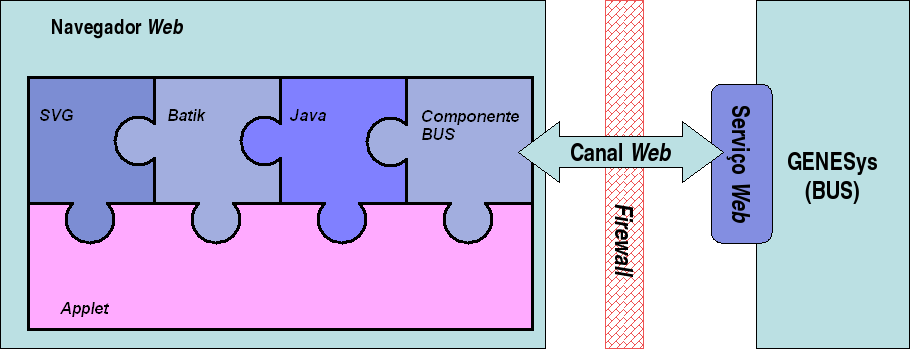
\includegraphics[width=0.86\textwidth]{puzzle}
    \caption{Proposed Architecture}
    \label{fig:arch}
  \end{center}
\end{figure}

Loren ipsum dolor sit amet, consectetuer adipiscing elit. 
Praesent sit amet sem. Maecenas eleifend facilisis leo. Vestibulum et
mi. Aliquam posuere, ante non tristique consectetuer, dui elit
scelerisque augue, eu vehicula nibh nisi ac est. Suspendisse elementum
sodales felis. Nullam laoreet fermentum urna. 

Pellentesque habitant morbi tristique senectus et netus et
malesuada fames ac turpis egestas. Fusce feugiat, elit ac placerat
fermentum, augue nisl ultricies eros, id fringilla enim sapien eu
felis. Vestibulum ante ipsum primis in faucibus orci luctus et
ultrices posuere cubilia Curae; Sed dolor mi, porttitor quis,
condimentum sed luctus. 

\subsection{Another subsection with  Tables}

Aenean rhoncus mauris sed ante tincidunt efficitur. Nam quis turpis
eleifend, rutrum nunc quis, interdum ipsum Table~\ref{tab:exemplo1}.
Suspendisse at sem nibh. Donec dapibus, lorem non faucibus dictum,
dolor sem porta mauris, id blandit nisl mi nec urna.
Suspendisse pretium diam massa Table~\ref{tab:exemplo2},
id tincidunt enim fringilla non. Ut posuere purus tortor, a dignissim
felis tempus gravida. Donec a facilisis nisi. Aliquam pulvinar lectus
sit amet libero fermentum, id blandit neque imperdiet. Phasellus
consequat blandit lacus ut bibendum. Integer eleifend condimentum
purus, vitae porttitor est. Ut vel ultrices nulla, quis volutpat quam.

\begin{table}[t]
  \centering
  \caption{A Simple Table}
\begin{tabular}{| l | l |}
	\hline
\textbf{Acronym} & \textbf{Description}\\
	\hline
	\hline
        ADT   & \emph{Abstract Data Type}\\\hline
        ANDF  & \emph{Architecture-Neutral Distribution Format}\\\hline
        API   & \emph{Application Programming Interface}\\
	\hline
\end{tabular}
  \label{tab:exemplo1}
\end{table}

Integer quis pede. Fusce nibh. Fusce nec erat vel mi condimentum
convallis. Sed at tortor non mauris pretium aliquet. In in lacus in
dolor molestie dapibus. Suspendisse potenti. Pellentesque sagittis
porta erat. Mauris sodales sapien id augue. Nam eu dolor. Donec sit
amet turpis non orci rhoncus commodo. Etiam condimentum commodo
libero.

Mauris pede. Curabitur faucibus dictum nibh. Proin tincidunt diam
vitae mauris. Sed hendrerit dolor vel ipsum. Nullam dapibus. Vivamus
tellus diam, egestas sit amet, vulputate non, vulputate id, eros. Nunc
sit amet nibh eget nibh imperdiet ornare. Cras vehicula mattis
ipsum. Sed diam arcu, semper at, gravida vitae, fermentum et,
nulla. Aenean massa orci, tristique nec, rutrum id, fringilla eget,
erat. Curabitur nulla ipsum, aliquam sed, rutrum vitae, semper quis,
ante. Fusce at nunc in dolor condimentum tempor. Duis sit amet massa. 

Curabitur convallis nulla quis risus. Nulla mollis porttitor
purus. Fusce ultricies odio at ligula pellentesque suscipit. Nulla
velit libero, blandit a, aliquet quis, hendrerit id, arcu. Phasellus
porttitor porttitor purus. Suspendisse velit tortor, fringilla sit
amet, commodo a, ultrices et, mi. Donec eu metus in erat ornare
adipiscing. Praesent varius mi ac nunc. Vestibulum leo lacus,
elementum in, vestibulum sit amet, hendrerit at, justo. Sed sit amet
neque. Donec libero risus, commodo sit amet, dignissim ut, tincidunt
a, eros. Ut non lacus quis tortor mattis ullamcorper. Vivamus
consequat augue vel erat. Sed tincidunt. Sed leo eros, ornare a,
pulvinar non, mattis quis, nibh. Aliquam faucibus mi ac nisi.

Pellentesque habitant morbi tristique senectus et netus et malesuada
fames ac turpis egestas. Duis aliquet, libero sit amet ornare viverra,
augue erat interdum dolor, vitae tincidunt lorem erat a lacus. Sed
lectus nisi, auctor in, hendrerit a, molestie vel, lectus. Cum sociis
natoque penatibus et magnis dis parturient montes, nascetur ridiculus
mus. Duis lacinia tempor dui. Vivamus rhoncus, tellus a viverra
dignissim, pede dui adipiscing odio, non faucibus metus mi gravida
eros. Nullam a tellus ut velit elementum tempus. Aenean rutrum
convallis tellus. Vestibulum nulla ante, dapibus ut, lobortis ut,
varius sed, nisl. Fusce lobortis. Sed ac lorem. Nulla tincidunt nulla
eget leo. Maecenas ac lectus eu neque ultrices pharetra. Curabitur a
risus nec arcu placerat tempor. Suspendisse magna nisl, viverra a,
adipiscing eget, ornare ultricies, ligula. Maecenas eu ligula vitae
eros convallis dignissim. 

\begin{table}[t]
  \centering
  \caption{A more Complex Table}
\begin{tabular}{|c|r@{.}lr@{.}lr@{.}l||r|}
	\hline
\multicolumn{8}{|c|}
	{\rule[-3mm]{0mm}{8mm}Iteration  $k$ of $f(x_n)$} \\
\textbf{\em k}
	& \multicolumn{2}{c}{$x_1^k$}
	& \multicolumn{2}{c}{$x_2^k$}
	& \multicolumn{2}{c||}{$x_3^k$}
	& comments \\ \hline \hline
0   & -0&3        & 0&6        &  0&7         & - \\
1   &  0&47102965 & 0&04883157 & -0&53345964  & $\delta<\epsilon$ \\
2   &  0&49988691 & 0&00228830 & -0&52246185  & $\delta < \varepsilon$ \\
3   &  0&49999976 & 0&00005380 & -0&523656    &   $N$ \\
4   &  0&5        & 0&00000307 & -0&52359743  & \\
\vdots	& \multicolumn{2}{c}{\vdots}
	& \multicolumn{2}{c}{$\ddots$}
	& \multicolumn{2}{c||}{\vdots}  & \\
7   &  0&5   & 0&0    & \textbf{-0}&\textbf{52359878}
		 & $\delta<10^{-8}$ \\ \hline
\end{tabular}
  \label{tab:exemplo2}
\end{table}

Loren ipsum dolor sit amet, consectetuer adipiscing elit. 
Praesent sit amet sem. Maecenas eleifend facilisis leo. Vestibulum et
mi. Aliquam posuere, ante non tristique consectetuer, dui elit
scelerisque augue, eu vehicula nibh nisi ac est. Suspendisse elementum
sodales felis. Nullam laoreet fermentum urna.  Cras vehicula mattis
ipsum. Sed diam arcu, semper at, gravida vitae, fermentum et,
nulla. Aenean massa orci, tristique nec, rutrum id, fringilla eget,
erat. Curabitur nulla ipsum, aliquam sed, rutrum vitae, semper quis,
ante. Fusce at nunc in dolor condimentum tempor

Duis eget diam. In est justo, tristique in, lacinia vel, feugiat eget,
quam. Pellentesque habitant morbi tristique senectus et netus et
malesuada fames ac turpis egestas. Fusce feugiat, elit ac placerat
fermentum, augue nisl ultricies eros, id fringilla enim sapien eu
felis. Vestibulum ante ipsum primis in faucibus orci luctus et
ultrices posuere cubilia Curae; Sed dolor mi, porttitor quis,
condimentum sed luctus. 

\section{Yet Another Section}

Loren ipsum dolor sit amet, consectetuer adipiscing elit. 
Praesent sit amet sem. Maecenas eleifend facilisis leo. Vestibulum et
mi. Aliquam posuere, ante non tristique consectetuer, dui elit
scelerisque augue, eu vehicula nibh nisi ac est. Suspendisse elementum
sodales felis. Nullam laoreet fermentum urna. 

Duis eget diam. In est justo, tristique in, lacinia vel, feugiat eget,
quam. Pellentesque habitant morbi tristique senectus et netus et
malesuada fames ac turpis egestas. Fusce feugiat, elit ac placerat
fermentum, augue nisl ultricies eros, id fringilla enim sapien eu
felis. Vestibulum ante ipsum primis in faucibus orci luctus et
ultrices posuere cubilia Curae; Sed dolor mi, porttitor quis,
condimentum sed luctus. 

\section{Summary}

Lorem ipsum dolor sit amet, consectetur adipiscing elit. Aliquam non
ultricies nibh, ut cursus neque. Vestibulum mattis ac odio ac
euismod. Integer posuere nibh odio, a fermentum massa iaculis
sed. 

Mauris eu mattis erat, eget feugiat quam. Fusce ut
justo sed lorem eleifend ornare ac vitae mi. Donec eu magna eget metus
porta vulputate. Aenean elementum turpis gravida elit iaculis
bibendum. 

\chapter{Experimental Study}\label{chap:chap4}



\section*{}
\section{SMART database considerations }
\paragraph{}This project consists of taking up the technique of diagnosing patients with DOC. For that, I had access to a dataset with 35 records of the assessment of this technique that took place in a hospital in London, where Professor Liliana Teixeira worked. Professor Liliana allowed me to access this dataset and was kind enough to explain how this technique works and clarify all the doubts that followed from reading the data and its particularities. The dataset has 147 columns of feature data. Many columns are repeated from 10 sessions that the technique uses for the evaluation of 8 modalities. There are 5 sensory modalities (gustatory, olfactory, auditory, visual and tactile), the rest are functional communication, wakefulness/arousal and motor function \cite{Gill-Thwaites2010}.
In this way, 8 modalities are evaluated in 10 times, making up 80 features that enlarge the data set. The multiple assessments of the same modality are, often, synonymous with feature redundancy.
The individual assessment of each session is done at the end of each session and this technique covers 2 evaluators, in 10 sessions and each of these is associated with the degree of certainty. In total we have over 40 columns/features.
In addition, there is a subsequent evaluation where the assessors discuss and reach a consensus on the joint result for each session and the associated degree of certainty. So we have 20 more features.
Of the other 7 features that remain, 2 are for patient identification and their evaluation order. These two features introduce noise to the model creation and not taken into consideration while creating supervised learning models.
Another 2 columns correspond to the y or diagnostic labels (in case of 2 and 3 possible states).
The labelling mode is shown in the following tables:
\begin{table}[!htb]
    
    \begin{minipage}{.5\linewidth}
      \caption{Classification with 2 states}
      \centering
       \begin{tabular}{|l|l|l|}
\hline

Label                 & Condition     & Quantity \\ \hline
1          & Vegetative State          & 10  \\ \hline 
2 & Minimally Conscious State        & 25  \\ \hline
\end{tabular}%
\label{tab:2StatesClassification}

\label{tab:Doc2states}
    \end{minipage}%
    \begin{minipage}{.5\linewidth}
      \centering
        \caption{Classification with 3 states}
        \begin{tabular}{|l|l|l|l}
\hline
Label & Condition & Quantity \\ \hline
1       & VS      & 10  \\ \hline
2      & MCS-     & 11  \\ \hline
3      & MCS+     & 14  \\ \hline
\end{tabular}%

\label{tab:DiagnosticLabeling}
    \end{minipage} 
\end{table}
\espaco
\espaco
\espaco
\espaco
\espaco
\espaco
\espaco
\espaco
\espaco
\espaco
\espaco
\espaco
\paragraph{}The \textbf{time} variable is the time interval, in months, between brain injury and SMART assessment. Age refers to the patient's age. These features are continuous, so, in the following table, you can check information about these: 

\begin{table}[ht]
\centering
\caption{Describe Age and Time}
\resizebox{.7\linewidth}{!}{%

\begin{tabular}{|l|l|l|l|l|}

\hline
Features & Mean & Minimum & Maximum & Median\\ \hline
Time (in months)     & 8,2  &3      & 70,0 & 52,0   \\ \hline
Age (in years)     & 49,7 & 19,0    & 77,0 & 6,0    \\ \hline
 
\end{tabular}%
}
\label{tab:Time&Age}
\end{table}

\paragraph{} The other two features are the patient's gender and the etiology/origin of the disease, they are binary with the following meaning:
\begin{table}[!htb]
    
    \begin{minipage}{.5\linewidth}
      \caption{Gender code definition}
      \centering
       \begin{tabular}{|l|l|l|l}
       \cline{1-3}
Label & Gender & Quantity \\ \hline
1     & Female & 7  \\ \hline
2     & Male   & 28  \\ \hline
\end{tabular}%




\label{tab:Gender}
    \end{minipage}%
    \begin{minipage}{.5\linewidth}
      \centering
        \caption{Etiology code definition}
        \begin{tabular}{|l|l|l|l}
\hline

Label & Etiology      & Quantity \\ \hline
1     & Traumatic     & 11  \\ \hline
2     & Not traumatic & 24  \\ \hline
\end{tabular}%

\label{tab:Etiology}
    \end{minipage} 
\end{table}





\chapter{Conclusions and Future Work} \label{chap:concl}

\section*{}


\section{Data exploration and analysis}

Upon close examination of the data summary, we can surmise that the classification for the two states is unbalanced. \ref{tab:2StatesClassification} .

And it turns out that there are fields with null values, 111 in total. This happens when the patient is blind or the gustatory sensory system is not possible to assess. It happens in the situations like patients are fed through a gastric tube or other alternative feeding mechanisms such as transcheostemia, etc.
All 'NA' are changed and assigned a non-significant value: -1. 
The reason for doing so is that data is precious and scarce, and removing records would further shorten our dataset. If we do not have sufficient. 
Without data, you cannot make the algorithm make a perfect model.
The ID and order insignificant columns are removed.
And the column of the diagnosis made by human evaluators, our label, is separated from X for an isolated panda's series y.

\section{Machine Learning}

X and y are split into training and testing subsets.
Taking care to stratify the data in relation to the label (stratify=y).
This is to ensure that all classes are proportional in relation to the training side to the testing side, avoiding the risk of poorly trained classes.
\clearpage

\section{Results}

The project repository is available at: https://github.com/ManJ-PC/ML-DoC

\espaco
\begin{figure}[ht] \centering 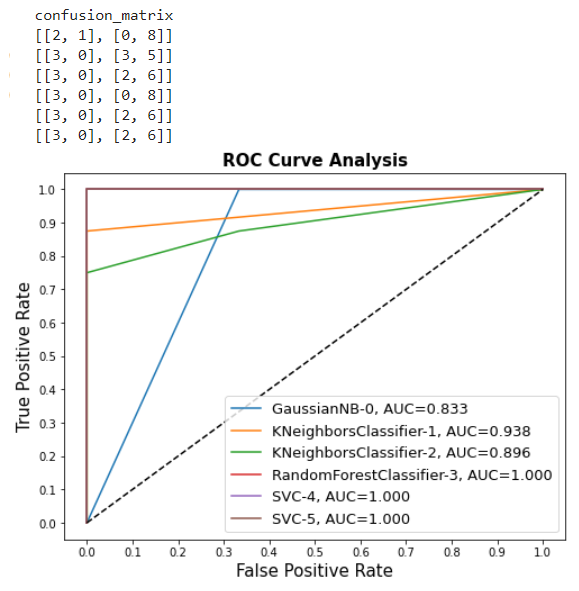
\includegraphics[scale=0.5]{figures/Results.png} 
\caption{Confusion Matrix and ROC curve of a Bunch of Algorithms} \label{fig:results}
 \end{figure}
 

\begin{figure}[ht] \centering 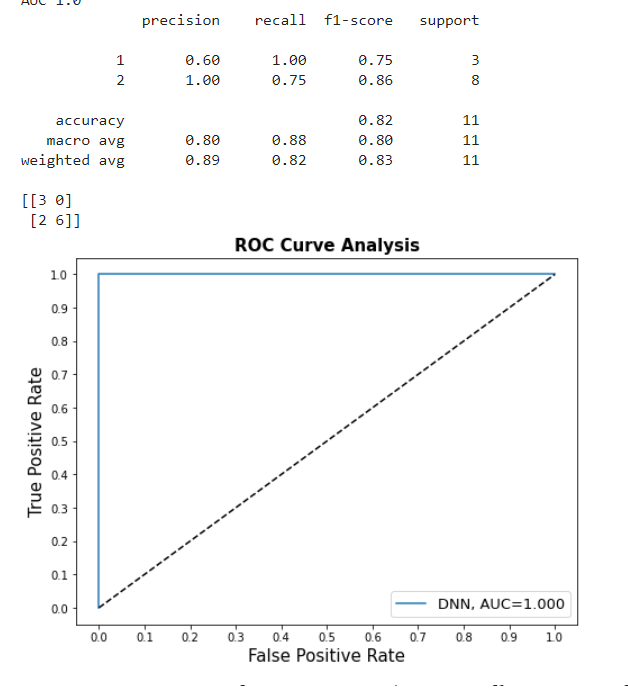
\includegraphics[scale=0.5]{figures/ResultsNN.png} 
\caption{Neural Network, Confusion Matrix and ROC curve resulting from the iterative method with 100 epochs, 25 neurons and ADAM optimizer} \label{fig:resultsNN}
 \end{figure}
 

\section{Further Work}



The project can be futher developed to find correlation of features in algorithms. Divide in two subgroups based on etiology. We can also see if it is possible to do less sessions to minimize resources of this tecnique(human resources, time spend). Since it may no longer be adding added value to the data.
\begin{itemize}
\item A broader view of classification in 3 possible stages (vegetative state, minimal state of consciousness minus and plus)
\item Iterate over the various machine learning algorithms
\item Unification of similar features \cite{9202409}
\item Predict the correlation of selected features and limit the number of sessions needed
\item Use of diagnostic tools to sensory data acquisition
\item Test the model with new and real data where it does not contain as rather sessions
\item Automate the entire process, acquire technological tools that allow you to track patients regularly
\end{itemize}


\vspace*{12mm}


 

%% comment next 2 commands if numbered appendices are not used
\appendix
\chapter{Loren Ipsum} \label{ap1:loren}

Coma (from the Greek kôma = deep sleep) can be defined as a state of total or partial loss of consciousness, voluntary motor skills and sensitivity, generally due to brain damage, intoxications, metabolic and endocrine problems, without which, regardless of severity, vital functions are maintained to a greater or lesser degree (1). When physiological, the state of coma can be measured using the Glasgow Coma Scale (GCSl) and when pharmacological using the Ramsay Sedation Scale (RSS).

\section{What is \emph{Loren Ipsum}?}

\emph{\textbf{Lorem Ipsum}} is simply dummy text of the printing and
typesetting industry. Lorem Ipsum has been the industry's standard
dummy text ever since the 1500s, when an unknown printer took a galley
of type and scrambled it to make a type specimen book.
It has survived not only five centuries, but also the leap into
electronic typesetting, remaining essentially unchanged.
It was popularised in the 1960s with the release of Letraset sheets
containing Lorem Ipsum passages, and more recently with desktop
publishing software like Aldus PageMaker including versions of Lorem
Ipsum\footnote{Available at \url{http://www.lipsum.com/}}.

\section{Where does Loren come from?}

Contrary to popular belief, Lorem Ipsum is not simply random text.
It has roots in a piece of classical Latin literature from 45 BC,
making it over 2000 years old.
Richard McClintock, a Latin professor at Hampden-Sydney College in
Virginia, looked up one of the more obscure Latin words, consectetur,
from a Lorem Ipsum passage, and going through the cites of the word in
classical literature, discovered the undoubtable source.
Lorem Ipsum comes from sections 1.10.32 and 1.10.33 of ``de Finibus
Bonorum et Malorum'' (The Extremes of Good and Evil) by Cicero,
written in 45 BC.
This book is a treatise on the theory of ethics, very popular during
the Renaissance. T
he first line of Lorem Ipsum, ``Lorem ipsum dolor sit amet\ldots'',
comes from a line in section 1.10.32.

The standard chunk of Lorem Ipsum used since the 1500s is reproduced
below for those interested.
Sections 1.10.32 and 1.10.33 from ``de Finibus Bonorum et Malorum'' by
Cicero are also reproduced in their exact original form, accompanied
by English versions from the 1914 translation by H. Rackham.

\section{Why using Loren?}

It is a long established fact that a reader will be distracted by the
readable content of a page when looking at its layout.
The point of using Lorem Ipsum is that it has a more-or-less normal
distribution of letters, as opposed to using ``Content here, content
here'', making it look like readable English.
Many desktop publishing packages and web page editors now use Lorem
Ipsum as their default model text, and a search for ``lorem ipsum''
will uncover many web sites still in their infancy.
Various versions have evolved over the years, sometimes by accident,
sometimes on purpose (injected humour and the like).  

\section{Where to Find Examples?}

There are many variations of passages of Lorem Ipsum available, but
the majority have suffered alteration in some form, by injected
humour, or randomised words which don't look even slightly
believable.
If you are going to use a passage of Lorem Ipsum, you need to be sure
there isn't anything embarrassing hidden in the middle of text.
All the Lorem Ipsum generators on the Internet tend to repeat
predefined chunks as necessary, making this the first true generator 
on the Internet.
It uses a dictionary of over 200 Latin words, combined with a handful
of model sentence structures, to generate Lorem Ipsum which looks
reasonable.
The generated Lorem Ipsum is therefore always free from repetition,
injected humour, or non-characteristic words etc. 


%%----------------------------------------
%% Final materials
%%----------------------------------------

%% Bibliography
%% Comment the next command if BibTeX file not used
%% bibliography is in ``myrefs.bib''
\PrintBib{myrefs}

%% Index
%% Uncomment next command if index is required
%% don't forget to run ``makeindex pdis'' command
%\PrintIndex

\end{document}
